\documentclass{article}
\usepackage{enumitem}
\usepackage[cachedir=minted_cache]{minted}
\usepackage{graphicx}
\graphicspath{ {./img/} }
\usepackage[margin=1in]{geometry} %used to set the margins
\setcounter{secnumdepth}{0} %used to get rid of section numbers
\title{INSERT TITLE}
\author{Michael Morikawa}
\date{\today}


\begin{document}
\maketitle
\section{Lab Questions}
\begin{enumerate}[label=\textbf{Question \arabic*}]
      \item  Outline an approach to represent an undirected graph using Edge List
            Structure. Try it out with a simple undirected graph with about 4 vertices and a few
            edges. \\
            \textbf{
                  In an Edge List Structure there are vertex objects stored in a collection; the vertices
                  simply store the element and the position in the collection. The edges contain an element
                  and the positions of the vertices that are the endpoints of the edge. So if we have a graph with
                  vertices A, B, C, D and edges 1, 2, 3. If edge 1 connects vertices A and B then in the edge object
                  it will store 1 as the element, and pointers to vertices A and B. Edge 2 connects B and C will be similar but
                  the endpoints will be pointing to B and C.
            }
      \item Discuss advantages of Adjacency List over Edge List Structure for an
            undirected graph.\\
            \textbf{
                  Adjacency List Structure runs faster than Edge List because it the list structure
                  we store in the vertices references to the edges incident to the vertex, and in
                  the edges we store the endpoint vertices for the edge. This allows for faster calculation
                  of the incident edges of a vertex, and determining if a vertex is adjecnt to another. Instead
                  of being proportional to the number of edges like in the edge list it is proportional to the
                  degree of the vertex.
            }


\end{enumerate}

\section{Source Code}

\subsection{AdjacencyListGraph.hpp}
\inputminted{c++}{../include/AdjacencyListGraph.hpp}
\subsection{testGraph.cpp}
\inputminted{c++}{../src/testGraph.cpp}

\section{Output}
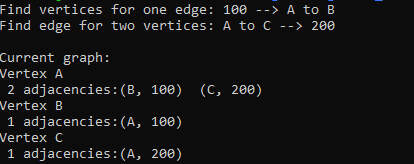
\includegraphics[]{output.png}

\end{document}